\documentclass[dvipsnames,png,border=10pt,tikz]{article}
\usepackage{tikz}
\usetikzlibrary{shapes.geometric} % required for the ellipse shape
%\usetikzlibrary{arrows, backgrounds, calc, hobby, positioning}



\usepackage{pgf}
\usepackage{tikz}
\usetikzlibrary{calc,arrows,decorations.pathmorphing,backgrounds,positioning,fit,petri,automata,shadings,shadows}


\tikzset{vertex style/.style={
    draw=#1,
    thick,
    fill=#1!70,
    text=white,
    ellipse,
    minimum width=2cm,
    minimum height=0.75cm,
    font=\small,
    outer sep=3pt,
  },
  text style/.style={
    sloped,
    text=black,
    font=\footnotesize,
    above
  }
}

\begin{document}
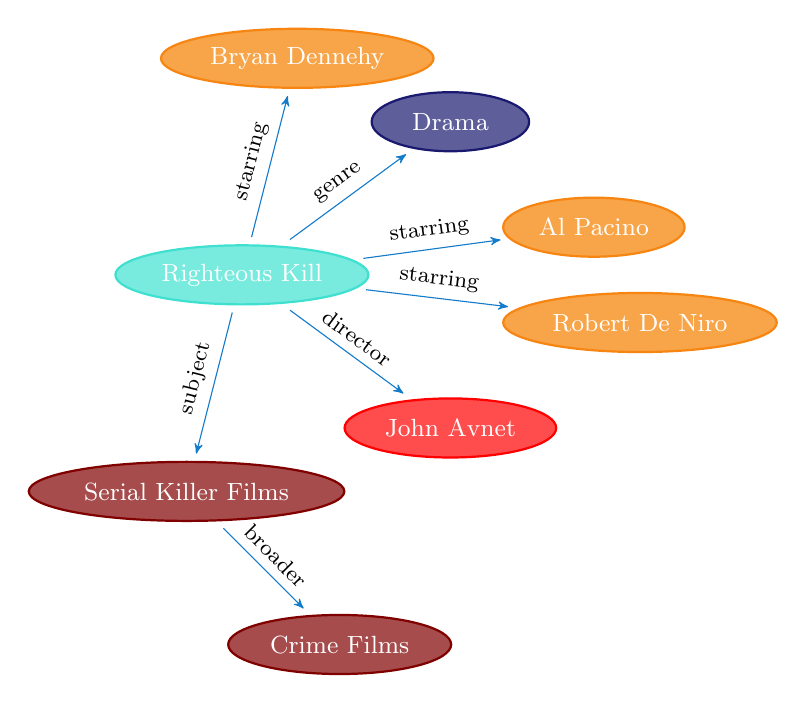
\begin{tikzpicture}[node distance=2.75cm,>=stealth']
\node[vertex style=Turquoise] (Rk) {Righteous Kill};

\node[vertex style=BurntOrange, above of=Rk,xshift=2em] (BD) {Bryan Dennehy}
 edge [<-,cyan!60!blue] node[text style]{starring} (Rk);

\node[vertex style=BurntOrange, right=1.5cm of Rk,yshift=4ex] (AP) {Al Pacino}
 edge [<-,cyan!60!blue] node[text style]{starring} (Rk); 

\node[vertex style=red, below right of=Rk,xshift=2em] (JA) {John Avnet}
 edge [<-,cyan!60!blue] node[text style]{director} (Rk); 

 \node[vertex style=BurntOrange, right=1.5cm of Rk,yshift=-4ex] (RN) {Robert De Niro}
 edge [<-,cyan!60!blue] node[text style]{starring} (Rk); 

\node[vertex style=MidnightBlue, above right of=Rk,xshift=2em] (Dr) {Drama}
 edge [<-,cyan!60!blue] node[text style]{genre} (Rk); 

\node[vertex style=Maroon, below of=Rk,xshift=-2em] (Skf) {Serial Killer Films}
 edge [<-,cyan!60!blue] node[text style]{subject} (Rk);

\node[vertex style=Maroon, below right of=Skf] (Cf) {Crime Films}
 edge [<-,cyan!60!blue] node[text style]{broader} (Skf);


\end{tikzpicture}




\end{document}